\def\bmode{0} % Mode 0 for presentation, mode 1 for a handout with notes, mode 2 fo% r handout without notes
\if 0\bmode
\documentclass[usenames,dvipsnames,smaller, hyperref={colorlinks=true,urlcolor=magenta,citecolor=cyan,linkcolor=orange}]{beamer}
\else \if 1\bmode
\immediate\write18{pdflatex -jobname=\jobname-Handout-Notes\space\jobname}
\documentclass[usenames,dvipsnames,smaller,handout,hyperref={colorlinks=true,urlcolor=magenta,citecolor=cyan,linkcolor=orange}]{beamer}
\usepackage{handoutWithNotes}
\pgfpagesuselayout{2 on 1 with notes}[letterpaper, landscape, border shrink=4mm]
\else \if 2\bmode
\immediate\write18{pdflatex -jobname=\jobname-Handout\space\jobname}
\documentclass[usenames,dvipsnames,smaller,handout,hyperref={colorlinks=true,urlcolor=magenta,citecolor=cyan,linkcolor=orange}]{beamer}
\fi
\fi
\fi

% \documentclass[smaller,handout
% ]{beamer}
%\usepackage{etex}
%\newcommand{\num}{6{} }

% \usetheme[
%   outer/progressbar=foot,
%   outer/numbering=counter,
%  block=fill
% ]{metropolis}

%\useoutertheme{metropolis}

\usetheme{Madrid}
\useoutertheme[subsection=false]{miniframes} % Alternatively: miniframes, infolines, split
\useinnertheme{circles}
\usecolortheme{seahorse}

\usepackage[backend=biber,style=authoryear,maxcitenames=2,maxbibnames=99,safeinputenc,url=false,
eprint=false]{biblatex}
%\addbibresource{bib/references.bib}
\AtEveryCitekey{\iffootnote{{\tiny}\tiny}{\tiny}}

%\usepackage{pgfpages}
%\setbeameroption{hide notes} % Only slides
%\setbeameroption{show only notes} % Only notes
%\setbeameroption{hide notes} % Only notes
%\setbeameroption{show notes on second screen=right} % Both

% \usepackage[sfdefault]{Fira Sans}

% \setsansfont[BoldFont={Fira Sans}]{Fira Sans Light}
% \setmonofont{Fira Mono}

%\usepackage{fira}
%\setsansfont{Fira}
%\setmonofont{Fira Mono}
% To give a presentation with the Skim reader (http://skim-app.sourceforge.net) on OSX so
% that you see the notes on your laptop and the slides on the projector, do the following:
% 
% 1. Generate just the presentation (hide notes) and save to slides.pdf
% 2. Generate onlt the notes (show only nodes) and save to notes.pdf
% 3. With Skim open both slides.pdf and notes.pdf
% 4. Click on slides.pdf to bring it to front.
% 5. In Skim, under "View -> Presentation Option -> Synhcronized Noted Document"
%    select notes.pdf.
% 6. Now as you move around in slides.pdf the notes.pdf file will follow you.
% 7. Arrange windows so that notes.pdf is in full screen mode on your laptop
%    and slides.pdf is in presentation mode on the projector.

% Give a slight yellow tint to the notes page
%\setbeamertemplate{note page}{\pagecolor{yellow!5}\insertnote}\usepackage{palatino}


%\usetheme{metropolis}
%\usecolortheme{beaver}
%\usepackage{xcolor}
\definecolor{darkcandyapplered}{HTML}{A40000}
\definecolor{lightcandyapplered}{HTML}{e74c3c}

%\setbeamercolor{title}{fg=darkcandyapplered}
%\setbeamercolor{frametitle}{bg=darkcandyapplered!80!black!90!white}
%\setbeamertemplate{frametitle}{\bf\insertframetitle}
%\setbeamercolor{footnote mark}{fg=darkcandyapplered}
%\setbeamercolor{footnote}{fg=darkcandyapplered!70}
%\Raggedbottom
%\setbeamerfont{page number in head/foot}{size=\tiny}
%\usepackage[tracking]{microtype}


\setbeamertemplate{frametitle}{%
    \nointerlineskip%
    \begin{beamercolorbox}[wd=\paperwidth,ht=2.0ex,dp=0.6ex]{frametitle}
        \hspace*{1ex}\insertframetitle%
    \end{beamercolorbox}%
}



\setbeamerfont{caption}{size=\footnotesize}
\setbeamercolor{caption name}{fg=darkcandyapplered}


%\usepackage[sc,osf]{mathpazo}   % With old-style figures and real smallcaps.
%\linespread{1.025}              % Palatino leads a little more leading

% Euler for math and numbers
%\usepackage[euler-digits,small]{eulervm}
%\AtBeginDocument{\renewcommand{\hbar}{\hslash}}
\usepackage{graphicx,multirow,paralist,booktabs}


%\mode<presentation> { \setbeamercovered{transparent} }

\setbeamertemplate{navigation symbols}{}
\makeatletter
\def\beamerorig@set@color{%
  \pdfliteral{\current@color}%
  \aftergroup\reset@color
}
\def\beamerorig@reset@color{\pdfliteral{\current@color}}
\makeatother

%=== GRAPHICS PATH ===========
\graphicspath{{./m2-images/}}
% Marginpar width
%Marginpar width
%\setlength{\marginparsep}{.02in}


%% Captions
% \usepackage{caption}
% \captionsetup{
%   labelsep=quad,
%   justification=raggedright,
%   labelfont=sc
% }

%AMS-TeX packages

\usepackage{amssymb,amsmath,amsthm} 
\usepackage{bm}
\usepackage{color}

\usepackage{hyperref,enumerate}
\usepackage{minitoc,array}


%https://tex.stackexchange.com/a/31370/2269
\usepackage{mathtools,cancel}

\renewcommand{\CancelColor}{\color{red}} %change cancel color to red

\makeatletter
\let\my@cancelto\cancelto %copy over the original cancelto command
\newcommand<>{\cancelto}[2]{\alt#3{\my@cancelto{#1}{#2}}{\mathrlap{#2}\phantom{\my@cancelto{#1}{#2}}}}
% redefine the cancelto command, using \phantom to assure that the
% result doesn't wiggle up and down with and without the arrow
\makeatother


\definecolor{slblue}{rgb}{0,.3,.62}
\hypersetup{
    colorlinks,%
    citecolor=blue,%
    filecolor=blue,%
    linkcolor=blue,
    urlcolor=slblue
}

%%%TIKZ
\usepackage{tikz}
\usepackage{pgfplots}
\usepackage{pgfplotstable}
\usepackage{pgfgantt}
\pgfplotsset{compat=newest}

\usetikzlibrary{arrows,shapes,positioning,shapes.geometric}
\usetikzlibrary{decorations.markings}
\usetikzlibrary{shadows,automata}
\usetikzlibrary{patterns}
\usetikzlibrary{trees,mindmap,backgrounds}
%\usetikzlibrary{circuits.ee.IEC}
\usetikzlibrary{decorations.text}
% For Sagnac Picture
\usetikzlibrary{%
    decorations.pathreplacing,%
    decorations.pathmorphing%
}
\tikzset{no shadows/.style={general shadow/.style=}}
%
%\usepackage{paralist}


%%% FORMAT PYTHON CODE
%\usepackage{listings}
% Default fixed font does not support bold face
\DeclareFixedFont{\ttb}{T1}{txtt}{bx}{n}{8} % for bold
\DeclareFixedFont{\ttm}{T1}{txtt}{m}{n}{8}  % for normal

% Custom colors
\definecolor{deepblue}{rgb}{0,0,0.5}
\definecolor{deepred}{rgb}{0.6,0,0}
\definecolor{deepgreen}{rgb}{0,0.5,0}

%\usepackage{listings}

% Python style for highlighting
% \newcommand\pythonstyle{\lstset{
% language=Python,
% basicstyle=\footnotesize\ttm,
% otherkeywords={self},             % Add keywords here
% keywordstyle=\footnotesize\ttb\color{deepblue},
% emph={MyClass,__init__},          % Custom highlighting
% emphstyle=\footnotesize\ttb\color{deepred},    % Custom highlighting style
% stringstyle=\color{deepgreen},
% frame=tb,                         % Any extra options here
    % showstringspaces=false            % 
% }}

% % Python environment
% \lstnewenvironment{python}[1][]
% {
% \pythonstyle
% \lstset{#1}
% }
% {}

% % Python for external files
% \newcommand\pythonexternal[2][]{{
% \pythonstyle
% \lstinputlisting[#1]{#2}}}

% Python for inline
% 
% \newcommand\pythoninline[1]{{\pythonstyle\lstinline!#1!}}


\newcommand{\osn}{\oldstylenums}
\newcommand{\dg}{^{\circ}}
\newcommand{\lt}{\left}
\newcommand{\rt}{\right}
\newcommand{\pt}{\phantom}
\newcommand{\tf}{\therefore}
\newcommand{\?}{\stackrel{?}{=}}
\newcommand{\fr}{\frac}
\newcommand{\dfr}{\dfrac}
\newcommand{\ul}{\underline}
\newcommand{\tn}{\tabularnewline}
\newcommand{\nl}{\newline}
\newcommand\relph[1]{\mathrel{\phantom{#1}}}
\newcommand{\cm}{\checkmark}
\newcommand{\ol}{\overline}
\newcommand{\rd}{\color{red}}
\newcommand{\bl}{\color{blue}}
\newcommand{\pl}{\color{purple}}
\newcommand{\og}{\color{orange!90!black}}
\newcommand{\gr}{\color{green!40!black}}
\newcommand{\nin}{\noindent}
\newcommand{\la}{\lambda}
\renewcommand{\th}{\theta}
\newcommand{\al}{\alpha}
\newcommand{\G}{\Gamma}
\newcommand*\circled[1]{\tikz[baseline=(char.base)]{
            \node[shape=circle,draw,thick,inner sep=1pt] (char) {\small #1};}}

\newcommand{\bc}{\begin{compactenum}[\quad--]}
\newcommand{\ec}{\end{compactenum}}

\newcommand{\p}{\partial}
\newcommand{\pd}[2]{\frac{\partial{#1}}{\partial{#2}}}
\newcommand{\dpd}[2]{\dfrac{\partial{#1}}{\partial{#2}}}
\newcommand{\pdd}[2]{\frac{\partial^2{#1}}{\partial{#2}^2}}



%%%%%%%%%%%%%%%%%%%%%%%%%%%%%%%%%%%%%%%%%%%%%%%%%%%
%%%%%%%%%%%%%%%%%%%%%%%%%%%%%%%%%%%%%%%%%%%%%%%%%%%

\title[CEE 260/MIE 273 2a: Events \& Set Operations]{{\normalsize CEE 260/MIE 273: Probability and Statistics in Civil Engineering} \\
Lecture 2a: Events and Set Operations}
\date[\today]{\footnotesize \today}
\author{{\bf Prof.\ Oke}}
\institute[UMass Amherst]{
  \begin{tikzpicture}[baseline=(current bounding box.center)]
    \node[anchor=base] at (-7,0) (its) {\includegraphics[scale=.3]{UMassEngineering_vert}} ;
  \end{tikzpicture}
}



%https://tex.stackexchange.com/questions/55806/mindmap-tikzpicture-in-beamer-reveal-step-by-step
  % \tikzset{
  %   invisible/.style={opacity=0},
  %   visible on/.style={alt={#1{}{invisible}}},
  %   alt/.code args={<#1>#2#3}{%
  %     \alt<#1>{\pgfkeysalso{#2}}{\pgfkeysalso{#3}} % \pgfkeysalso doesn't change the path
  %   },
  % }


\usepackage{listings}

\lstset{language=matlab,
                basicstyle=\scriptsize\ttfamily,
                keywordstyle=\color{blue}\ttfamily,
                stringstyle=\color{blue}\ttfamily,
                commentstyle=\color{gray}\ttfamily,
                morecomment=[l][\color{gray}]{\#}
              }
         
\begin{document}

\maketitle




\begin{frame}
  \frametitle{Outline}
  \tableofcontents
\end{frame}


\begin{frame}
  \frametitle{Module 2: Probability}
  \pause
  Key goals for this module: \pause

  \begin{itemize}
  \item Understand basic set theory and operations \pause
  \item Understand introductory  probability theory \pause
  \item Learn the fundamentals of conditional probability and Bayes' theorem
  \end{itemize}
\end{frame}

\begin{frame}
  \frametitle{Objectives of today's lecture}
  \pause

  \begin{itemize}[<+->]
  \item Learn the fundamentals of set theory and operations
  \item Understand events and sample spaces
  \item Use set theory to express combinations of events
  \item Understand the concepts of mutual exclusivity and collective exhaustivity of events
  %\item Learn and apply De Morgan's Rule
  \end{itemize}
\end{frame}


  
\section{Elements of set theory}

\begin{frame}
  \frametitle{Reals, rationals, integers and natural numbers}\pause
  
    \begin{itemize}[<+->]
    \item  A \textbf{real} number is the value of a continuous quantity that can either be expressed as an infinite decimal expansion or on a number line.\\
      
      \pause
      The set of  real numbers is denoted by $\mathbb{R}$ and it is the superset of rational and irrational numbers.

      \bigskip
      
    \item A \textbf{rational} number can be expressed as a fraction of two integers.\\ \pause
      The set of rational numbers is denoted by $\mathbb{Q}$

      \bigskip
      
    \item The set of \textbf{integers} $\{\ldots, -2, -1, 0, 1, 2, \ldots\}$ is denoted by $\mathbb{Z}$. \\ \pause
      It is the superset of natural numbers.

      \bigskip
    \item The set of \textbf{natural} numbers (used for counting) is denoted by $\mathbb{N}$.
  \end{itemize}

  \pause
  \begin{alertblock}{}
  \begin{equation}
    \mathbb{N} \subset     \pause \mathbb{Z} \subset \pause     \mathbb{Q} \subset   \pause  \mathbb{R} 
  \end{equation}
  \pause
  The symbol ``$\subset$'' means ``is a subset of''
\end{alertblock}

\end{frame}
\begin{frame}
  \frametitle{Key definitions}\pause
  Set theory provides tools for characterizing sample spaces and thus formulating probabilistic problems.

  \pause
  \bigskip
  
%  \begin{block}{Key definitions}
  \begin{description}[labelwidth=10ex]
  \item[Sample space:] A collection of individual possibilities ({\it sample points}) \pause
  \item[Event:] A subset of the sample space  \pause
  \item[Finite set:] has 1-1 correspondence with a \textbf{bounded subset} of natural numbers $\mathbb{N} = \{1,2,3,\ldots\}$ \pause
  \item[Countable set:] has 1-1 correspondence with a \textbf{subset} of natural numbers $\mathbb{N}$  \pause
  \item[Infinite set:] has 1-1 correspondence with an \textbf{unbounded set} of real numbers  $\mathbb{R}$\pause
  \item[Uncountable set:] has 1-1 correspondence with the \textbf{entire set} of real numbers $\mathbb{R}$ 
  \end{description}
  % \end{block} 
\end{frame}

\begin{frame}
  \frametitle{Sample spaces}
  \pause
 % \begin{alertblock}{Key implications}
  \begin{itemize}[<+->]
  \item A sample space may be:
    \begin{enumerate}[<+->]   
    \item Discrete (countable sample points---finite or infinite) 
    \item Continuous (uncountable/infinite)  
    \end{enumerate}
    
  \item All \textbf{\bl uncountable} sets are \textbf{\bl infinite} \pause
    \begin{itemize}
    \item e.g.\ the set of real numbers $\mathbb{R}$
    \end{itemize}

  \item A continuous sample space is infinite
  \item A \textit{\pl countably infinite} set is both countable and infinite, \pause e.g.
    \begin{itemize}[<+->]
    \item  the set of natural numbers $\mathbb{N} = \{1,2,3,\ldots\}$
    \item the set of integers $\mathbb{Z} = \{\ldots, -2, -1, 0, 1, 2, \ldots\}$
  \end{itemize}

  \end{itemize}
  % \end{alertblock}

  \pause

  \bigskip
  
  \begin{center}
    \begin{tabular}{| c | c | c |}\hline
      & \bf Countable & \bf Uncountable \\ \hline       
      \bf Finite    & Discrete  & ---  \\ \hline
      \bf Infinite  & Discrete  & Continuous \\\hline
    \end{tabular}
  \end{center}

\end{frame}

\begin{frame}
  \frametitle{Example 1: Characterizing sample spaces }\pause

  \bigskip
  
  Characterize the following  as  {\it finite discrete}, {\it infinite discrete} or {\it continuous}: \pause

  \bigskip
  
\begin{itemize}%[<+->] 
    \item Number of flaws in a given length of welding. \pause \alert{\it infinite discrete}\pause

    \item Total number of flights departing from Bradley International Airport in a given day. \pause \alert{\it finite discrete} \pause

    \item Arrival time of passenger in metro station relative to departure of
      last train $[0,T]$, where $T$ is the interval between two consecutive
      trains. \pause \alert{\it continuous} \pause

    \item The number of days in a year with potentially measurable precipitation
      in Seattle. \pause \alert{\it finite discrete}
    \end{itemize}

\end{frame}



\section{Set operations and properties}
\begin{frame}
  \frametitle{Set notation} \pause
  
  
  \begin{table}
    \centering
    \begin{tabular}{l l}\toprule
    \bf Symbol & \bf Meaning \\ \midrule  \pause
      $\cup$ & union \\ \pause
      $\cap$ & intersection \\ \midrule \pause 
      $\supset$ & proper superset \\\pause
      $\subset$ & proper subset \\\pause
      $\supseteq$ &  superset or equal to \\\pause
      $\subseteq$ & subset  or equal to \\ \midrule \pause
      $\overline{E}$ or $E^{c}$& complement of $E$ \\\pause
      $\varnothing$ & empty/null set\\ \bottomrule
    \end{tabular}
\end{table}

\end{frame}

\begin{frame}
  \frametitle{Set equality} \pause
  Given a set $A$ and sample space $S$:  \pause
  
  \begin{eqnarray}
    A \cup \varnothing &=& A \\ \pause
    A \cap \varnothing &=& \varnothing \\   \pause
    A \cup A &=& A \\  \pause
    A \cap A &=& A \\  \pause
    A \cup S &=& S \\  \pause
    A \cap S &=& A 
  \end{eqnarray}
  \pause

  \begin{itemize}[<+->]
  \item The union or intersection of a set with itself yields the same set
  \item The intersection of a set with the empty set yields the empty set
  \item \dots
  \end{itemize}
\end{frame}





\begin{frame}
  \frametitle{Set properties: union and intersection}

  \begin{block}{Commutative property} \pause
    \begin{eqnarray}
      A \cup B &=&B \cup A \\ \pause
      A \cap B &=&B \cap A
    \end{eqnarray}
  \end{block}

  \pause
  \begin{block}{Associative property}\pause
    \begin{eqnarray}
      (A \cup B) \cup C &=&A \cup ( B \cup C) \\ \pause
      (AB)C &=&A(BC)
    \end{eqnarray}
  \end{block}

  \pause 
  \begin{block}{Distributive property}\pause
    \begin{eqnarray}
    (A \cup B) \cap C &=&(A \cap C) \cup (B \cap C)  \\\pause
      (AB) \cup C &=&(A\cup C) \cap (B \cup C)
    \end{eqnarray}
  \end{block}

\end{frame}


\begin{frame}
  \frametitle{Set properties: complements}\pause
  Given an event $E$ and a sample space $S$:
\pause
  \begin{eqnarray}
    E \cup \overline{E} &=& S \\  \pause
    E \cap \overline{E} &=& \varnothing \\  \pause
    \overline{\overline{E}} &=& E 
  \end{eqnarray}
\end{frame}

\begin{frame}
  \frametitle{Example 2: Set operations}
  \pause
  Given the sets:
  \begin{eqnarray*}
    A &=&\{1, 3, 8, 10\} \\ \pause
    B &=&\{0, 2, 5, 7, 10\}
  \end{eqnarray*}
  \pause

  Find:
  \begin{enumerate}[<+->]
  \item $A \cup B$ \pause (``$A$ union $B$''): \pause
    \begin{quote}
      \begin{eqnarray*}\gr
        A \cup B &=&\gr \{0, 1, 2, 3, 5, 7, 8, 10\}
      \end{eqnarray*}
    \end{quote}
    \pause

  \item $A \cap B$ \pause (``$A$ intersection $B$''): \pause
    \begin{quote}
      \begin{eqnarray*}\gr
        A \cap B &=&\gr \{10\}
      \end{eqnarray*}
    \end{quote}

  \item If the sample space is given by the integers in the interval $[0,10]$, find $(A\cup B)^{c}$: \pause
    \begin{quote}\gr
      \begin{eqnarray*}
        (A\cup B)^{c} &=& \pause \{4, 6, 9\}
      \end{eqnarray*}
    \end{quote}
  \end{enumerate}
\end{frame}

\begin{frame}
  \frametitle{Venn diagrams} \pause
  An approach for visualizing sets (sample spaces) and analyzing events. \pause

  \only<2->{
    \begin{exampleblock}{Venn diagram showing an event $E$ and its complement $\ol{E}$}\pause
      \only<3->{
        \begin{center}
          \begin{tikzpicture}[scale=.8]
            \only<4->{\draw[thick]  (-4,-3) rectangle (7,3) node[below left] {$\bm S$};}      
            \only<5->{\draw[thick, pattern=north west lines,pattern color=green!50!black] (1.5,0) circle (2 cm) node {$\bm{E}$};}
            \only<6->{\begin{scope}
                \draw[fill=red!20!]  (-4,-3) rectangle (7,3) ;
                \node[red] at (-2, 1) {$\bm{E^{c} \equiv \ol{E}}$} node[below left] {$\bm S$};
                \draw[fill=white,] (1.5,0) circle (2 cm);
                \draw[ pattern=north west lines,pattern color=green!50!black] (1.5,0) circle (2 cm) node {$\bm{E}$};
              \end{scope}}
          \end{tikzpicture}
        \end{center}
      }
    \end{exampleblock}
  }
\end{frame}


\begin{frame}
  \frametitle{Activity: Pizza Preference Survey}\pause

%(15-20 minutes, great for unions, intersections, and complements)
\begin{alertblock}{Setup}
  \begin{itemize}
    \item $A$ = students who like pepperoni
  \item $B$ = students who like mushrooms
\item $C$ = students who like pineapple
  \end{itemize}
\end{alertblock}


\pause
\begin{block}{Activity}
  \begin{itemize}
    \item Stand and sort yourselves physically into regions of the room
  \item Start with just sets $A$ and $B$, creating a human Venn diagram
  \item Add set $C$ and watch the complexity emerge
\item Count each region and calculate: $|A \cup B|$, $|A \cap B|$, 
$|A^c|$, $|B^c|$, $|C^c|$.
  \end{itemize}
\end{block}
\end{frame}


\section{Events}



\begin{frame}
  \frametitle{Events}\pause
  An event $E$ contains one or more sample points within a sample space $S$ \pause

  \bigskip
  
  \begin{itemize}[<+->]
  \item Events can be derived from other events by union or by intersection
  \item An \alert{impossible event} is an empty set $\varnothing$
  \item A \alert{certain event} contains all the sample points in a sample space\\
    \pause {\it What is the probability of a certain event?}
  \item A \alert{complementary event} $\overline{E}$ of an event $E$ contains all the sample points in $S$ not in $E$ \\
    \pause
    \begin{equation}
      \label{eq:1}
      \overline{E} = S\setminus E
    \end{equation}
  \end{itemize}
\end{frame}


\begin{frame}
  \frametitle{Union}
  \pause

  \begin{block}{Definition}
    The union of two events $E_1$ and $E_2$ (denoted $E_1 \cup E_2$) is the
    occurrence of $E_1$ or $E_2$ or both.
  \end{block}

  \pause

  \begin{center}
    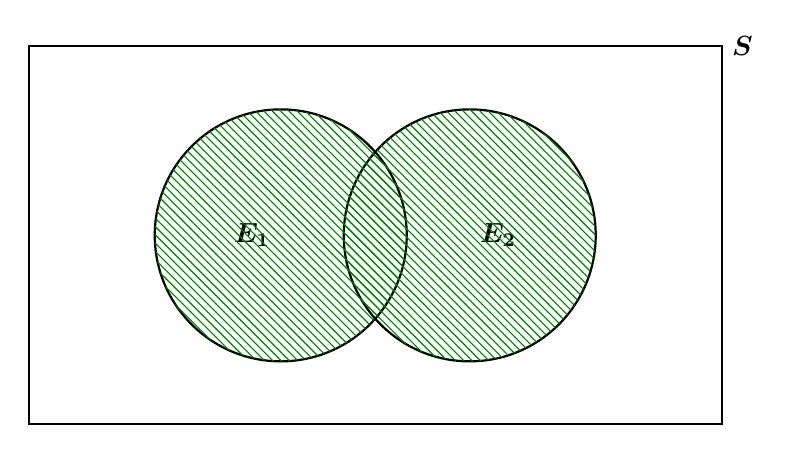
\begin{tikzpicture}[scale=.8]
      \visible<+->{\draw[thick]  (-4,-3) rectangle (7,3) node[anchor=north east, right] {$\bm S$};}
      \visible<+->{
        \draw[thick] (0,0) circle (2 cm) node[left] {$\bm{E_{1}}$};
        \draw[thick]  (3,0) circle (2 cm) node[right] {$\bm{E_{2}}$};
      }
    \visible<+->{
      \fill[pattern=north west lines,pattern color=green!50!black] (3,0) circle (2 cm);
      \fill[pattern=north west lines,pattern color=green!50!black](0,0) circle (2 cm);
    }
    \end{tikzpicture}
  \end{center}
\end{frame}

\begin{frame}
  \frametitle{Intersection}
      
  \begin{block}{Definition}
    The intersection of two events $E_1$ and $E_2$ (denoted $E_1 \cap E_2$  or $E_{1}E_{2}$) is the
    joint occurrence of $E_1$ and $E_2$.
  \end{block}

  \pause

  \begin{center}
  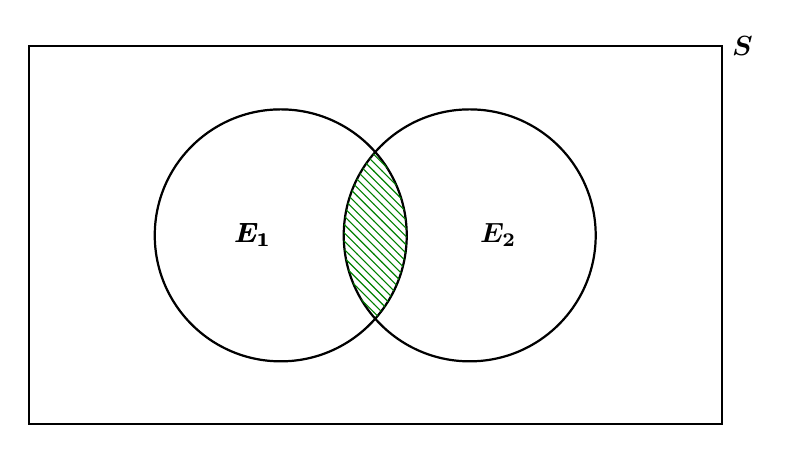
\begin{tikzpicture}[scale=.8]
    \visible<+->{\draw[thick]  (-4,-3) rectangle (7,3) node[anchor=north east, right] {$\bm S$};}
    \visible<+->{
      \draw[thick] (0,0) circle (2 cm) node[left] {$\bm{E_{1}}$};
      \draw[thick]  (3,0) circle (2 cm) node[right] {$\bm{E_{2}}$};
    }
    \visible<+->{
      \begin{scope}
        \clip[draw] (0,0) circle (2 cm) node[left] {$\bm{E_{1}}$};
        \fill[pattern=north west lines,pattern color=green!50!black]  (3,0) circle (2 cm);
      \end{scope}
    }
  \end{tikzpicture}
\end{center}
\end{frame}

\begin{frame}
  \frametitle{Mutually exclusive  events}

  \pause
  \begin{block}{Definition}
    Two or more events are mutually exclusive if the occurrence of one event
    precludes the occurrence of any or all of the others: \pause
    \begin{equation}
      \label{eq:4}
      E_1 \cap E_2 = \varnothing
    \end{equation}
  \end{block}

  \pause


   \begin{center}
    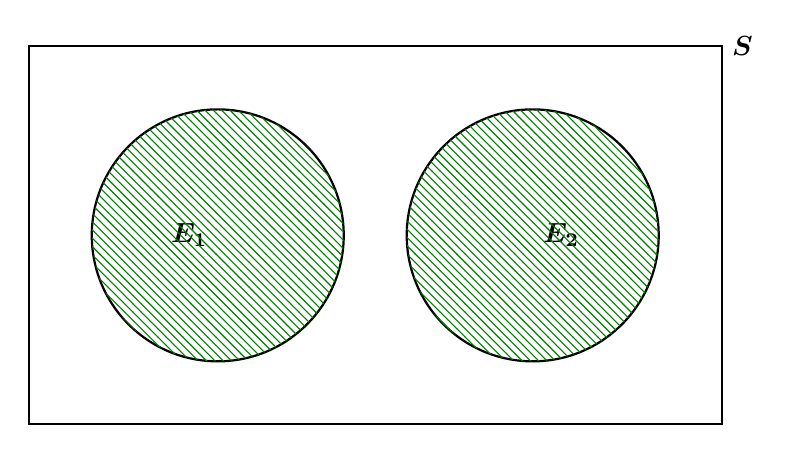
\begin{tikzpicture}[scale=.8]
      \visible<+->{\draw[thick]  (-4,-3) rectangle (7,3) node[anchor=north east, right] {$\bm S$};}
      \visible<+->{
        \draw[thick] (-1,0) circle (2 cm) node[left] {$\bm{E_{1}}$};
        \draw[thick]  (4,0) circle (2 cm) node[right] {$\bm{E_{2}}$};
      }
    \visible<+->{
      \fill[pattern=north west lines,pattern color=green!50!black] (4,0) circle (2 cm);
      \fill[pattern=north west lines,pattern color=green!50!black](-1,0) circle (2 cm);
    }
    \end{tikzpicture}
  \end{center}
\end{frame}

\begin{frame}
  \frametitle{Collectively exhaustive events}
\pause
\begin{block}{Definition}\pause
  A group of events are collectively exhaustive if their union is equal to the
  sample space containing the events. \pause $E_{1}\cup E_{2}\cup E_{3} = S$
\end{block}
\pause


   \begin{center}
    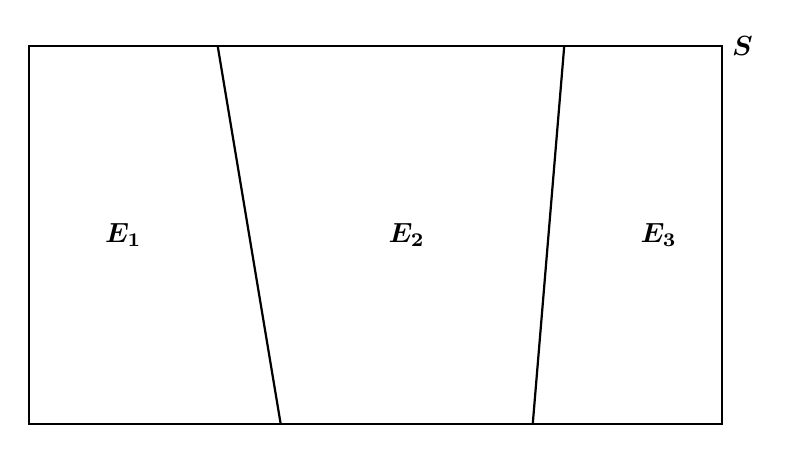
\begin{tikzpicture}[scale=.8]
      \visible<+->{\draw[thick]  (-4,-3) rectangle (7,3) node[anchor=north east, right] {$\bm S$};}
      \visible<+->{
        \draw[thick] (0,-3) -- (-1, 3) ;
        \draw[thick]  (4,-3) -- (4.5,3) ;
      }
    \visible<+->{
      \node at (-2.5,0) {$\bm{E_{1}}$};
      \node at (2,0) {$\bm{E_{2}}$};
      \node at (6,0) {$\bm{E_{3}}$};
    }
    \end{tikzpicture}
  \end{center}

\end{frame}


\begin{frame}
  \frametitle{Example 3:  Bidding for projects}

  \pause

  Two construction companies $a$ and $b$ are bidding for projects. Define $A$
    as the event that Company $a$ wins a bid, and $B$ likewise for $b$. Sketch
    the Venn diagrams and characterize the following events:

    \bigskip

    \pause
    
    \begin{enumerate}[(i)]
    \item Company $a$ submitting a bid for one project and Company $b$ submitting a bid for another project

    \item Companies $a$ and $b$ submitting bids for the same project.

    \item Company $a$ and company $b$ are the only bidders for the single project
    \end{enumerate}
\end{frame}

\begin{frame}
  \frametitle{Example 3: Bidding for projects (cont.)}

  (i) Company $a$ submitting a bid for one project and Company $b$ submitting
  a bid for another project: \pause 
  
  
  \begin{center}
    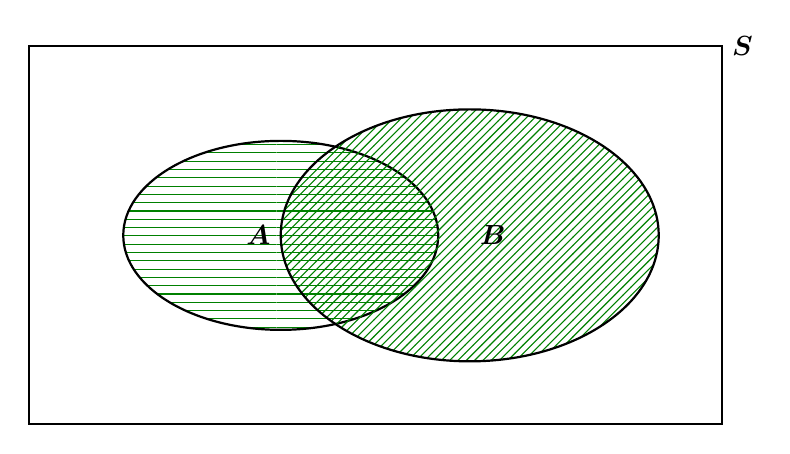
\begin{tikzpicture}[scale=.8]
      \visible<+->{\draw[thick]  (-4,-3) rectangle (7,3) node[anchor=north east, right] {$\bm S$};}
      \visible<+->{
        \draw[thick,pattern= horizontal lines,pattern color=green!50!black] (0,0) ellipse (2.5 cm and 1.5 cm ) node[left] {$\bm{A}$};
      }
      \visible<+->{
        \draw[thick,pattern= north east lines, pattern color=green!50!black]  (3,0) ellipse (3 cm and 2 cm) node[right] {$\bm{B}$};
      }
    \end{tikzpicture}
  \end{center}

\end{frame}

\begin{frame}
  \frametitle{Example 3: Bidding for projects (cont.)}
  \pause
  (ii) Companies $a$ and $b$ submitting bids for the same project. \pause

  
  \begin{center}
    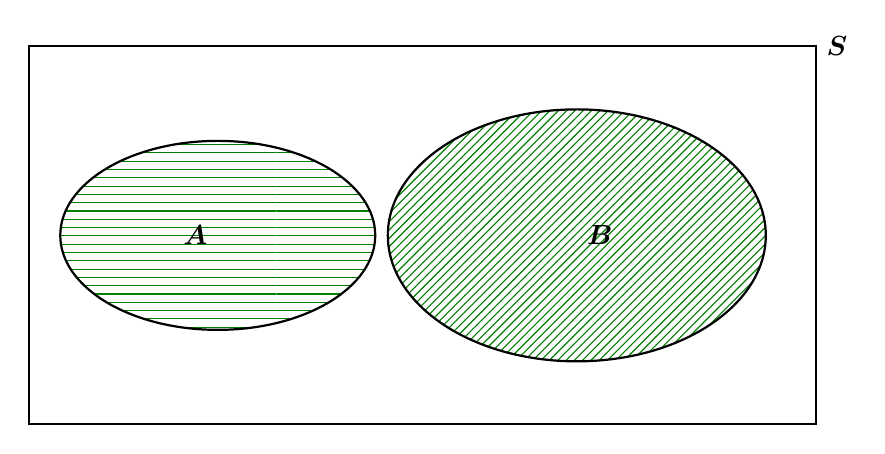
\begin{tikzpicture}[scale=.8]
      \visible<+->{\draw[thick]  (-4,-3) rectangle (8.5,3) node[anchor=north east, right] {$\bm S$};}
      \visible<+->{
        \draw[thick,pattern= horizontal lines,pattern color=green!50!black] (-1, 0) ellipse (2.5 cm and 1.5 cm ) node[left] {$\bm{A}$};
      }
      \visible<+->{
        \draw[thick,pattern= north east lines,pattern color=green!50!black]  (4.7, 0 ) ellipse (3 cm and 2 cm) node[right] {$\bm{B}$};
      }
    \end{tikzpicture}
  \end{center}
  \pause

  These events are mutually exclusive, as both companies cannot win the same project.
 \end{frame}

\begin{frame}
  \frametitle{Example 3: Bidding for projects (cont.)}

  \pause

  (iii) Company $a$ and company $b$ are the only bidders for the single project available.

  \pause


  \begin{center}
    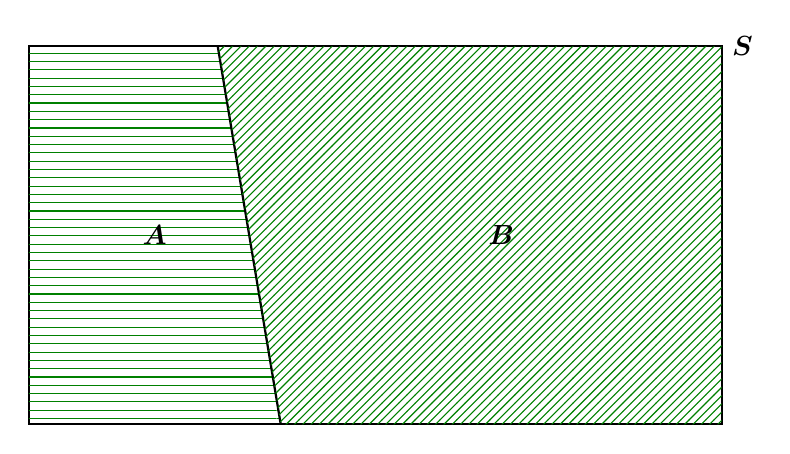
\begin{tikzpicture}[scale=.8]
      \visible<+->{\draw[thick]  (-4,-3) rectangle (7,3) node[anchor=north east, right] {$\bm S$};}
      \visible<+->{
        \fill[pattern=horizontal lines,pattern color=green!50!black] (-4,-3) -- (0,-3) -- (-1,3) -- (-4,3) -- cycle;
        \node  at  (-2, 0) {$\bm{A}$};
              \draw[thick] (0,-3) -- (-1,3) ;

      }
      \visible<+->{
        \fill[pattern=north east lines,pattern color=green!50!black] (0,-3) -- (7,-3) -- (7,3) -- (-1,3)  -- cycle;
        \node at (3.5,0) {$\bm{B}$};
      }
    \end{tikzpicture}
  \end{center}

  
  \pause

  These events are both mutually exclusive and collectively exhaustive.
 \end{frame}





\section{Outlook}
\begin{frame}
  \frametitle{Recap}
  \begin{itemize}[<+->]
  \item Set theory and operations: union, intersection, complement
  \item Events occur within a sample space of possibilities
  \item The sample space can be discrete or continuous
  \item Mutually exclusive events cannot jointly occur
  \item The union of collectively exhaustive events yields the sample space
  \item De Morgan's Rules are useful for expressing complements of unions or of intersections
  \end{itemize}

  Play around with set operations: \url{https://seeing-theory.brown.edu/compound-probability/index.html\#section1}
\end{frame}
 

\appendix\addtocounter{part}{-1}

\section{Appendix: De Morgan's Rule}
\begin{frame}
  \frametitle{De Morgan's rule}
  \pause
  \begin{block}{Complement of a union}\pause
    The complement of the union of a given number of sets/events is the intersection of their complements:
    \pause
    \begin{eqnarray}
      \ol{A \cup B} &=& \ol{A} \cap \ol{B} \\\pause
      \ol{A \cup B \cup C} &=& \ol{A} \cap \ol{B} \cap \ol{C}\\\pause
      \overline{E_1 \cup E_2 \cup \cdots \cup E_n} &=& \overline{E_1} \cap \overline{E_2} \cap \cdots \cap \overline{E_n}
    \end{eqnarray}
  \end{block}

  \pause

  Equivalently:
  \pause
  
 \visible<+->{ \begin{block}{Complement of an intersection }
    The complement of the intersection of a given number of sets/events is the union of their complements:
\pause
    \begin{eqnarray}
      \ol{A \cap B} = \pause \ol{AB} \pause  &=& \ol{A} \cup \ol{B} \\\pause
      \ol{ A \cap B \cap C} =\pause \ol{ABC} \pause  &=& \ol{A} \cup \ol{B} \cup \ol{C}\\\pause
      \overline{E_1 \cap E_2 \cap \cdots \cap E_n} &=& \overline{E_1} \cup \overline{E_2} \cup \cdots \cup \overline{E_n}
    \end{eqnarray}    
  \end{block}
}
\end{frame}


\begin{frame}
  \frametitle{Venn diagram demonstrating de Morgan's rule}
  \begin{center}
    \visible<+->{\includegraphics[width=.6\textwidth, trim={0 15cm 0 0},clip]{02_06}}
    \visible<+->{\includegraphics[width=.6\textwidth, trim={0 7.5cm 0 5cm}, clip]{02_06}}
    \visible<+->{\includegraphics[width=.6\textwidth, trim={0 1cm 0 13cm},clip]{02_06}}
\end{center}

\pause

$\ol{E_{1}\cup E_{2}} = \pause \ol{E_{1}} \cap \ol{E_{2}}$
\end{frame}

\begin{frame}
  \frametitle{Example 4: Water supply}
  \pause
  
    The water supply for two cities $C$ and $D$ comes from the two sources $A$
    and $B$. Water is transported by pipelines 1, 2, 3 and 4. Assume that either
    one of the two sources by itself is sufficient to supply the water for both
    cities. Also, denote $E_1, E_2, E_3, E_4$ as the failure of branches 1, 2, 3 and 4, respectively.

    \begin{center}
      \includegraphics[width=.6\textwidth, trim={0 2cm 0 0}, clip]{E_02_12}      
    \end{center}

    \pause
    \begin{enumerate}[\bf (a)]
    \item Denote the event that there is no shortage of water in $C$.
    \item Denote the event that there is no shortage of water in $D$.
    \end{enumerate}
    Simplify your answers using De Morgan's rule.
 \end{frame}


\begin{frame}
  \frametitle{Example 4: Water supply (cont.)}
    \begin{center}
      \includegraphics[width=.6\textwidth, trim={0 2cm 0 0}, clip]{E_02_12}      
    \end{center}

    \pause

    Shortage of water in $C$ is represented by \pause $E_1 \cap E_2 \cup E_3$. \pause
    Its complement $\overline{E_1E_2\cup E_3}$ means there is no shortage of water in $C$.
    \pause
    Applying de Morgan's rule, we have: \pause

    $\overline{E_1E_2\cup E_3} = \overline{E_1E_2}\cap \overline{E_3} = (\overline{E_1}\cup\overline{E_2})\overline{E_3}$
 \end{frame}

\begin{frame}
  \frametitle{Example 4: Water supply (cont.)}
 
    \pause

        \begin{center}
      \includegraphics[width=.6\textwidth, trim={0 2cm 0 0}, clip]{E_02_12}      
    \end{center}

    \pause
    
    No shortage of water in $D$ is represented by \pause $\overline{E_1E_2\cup E_3 \cup  E_4}$.\\
    \bigskip

    \pause Simplified using de Morgan's rule, this becomes \pause $(\overline{E_1}\cup \overline{E_2})\overline{E_3}\overline{E_4}$
 \end{frame}


%\begin{frame}[allowframebreaks]
%   \frametitle{References}
%   \AtNextBibliography{\scriptsize}
%   \setbeamertemplate{bibliography item}[text]
%   \printbibliography[heading=none]
  
% \end{frame}

%\printbibliography
\end{document}
%%% Local Variables:
%%% mode: latex
%%% TeX-master: t
%%% End:
